\documentclass[a4paper]{article}

%% Language and font encodings
\usepackage[english, russian]{babel}
\usepackage[utf8x]{inputenc}
\usepackage[T1]{fontenc}
\usepackage[showframe=false]{geometry}
\usepackage{changepage}

%% Sets page size and margins
\usepackage[a4paper,top=3cm,bottom=2cm,left=3cm,right=3cm,marginparwidth=1.75cm]{geometry}

%% Useful packages
\usepackage{amsmath}
\usepackage{graphicx}
\usepackage[colorinlistoftodos]{todonotes}
\usepackage[colorlinks=true, allcolors=blue]{hyperref}
\title{Работа 2.2.6 Определение энергии активации
	по температурной зависимости вязкости жидкости}
\author{Дмитриева Ирина, 597 группа}
\date{}
\begin{document}
\maketitle
	
	% \begin{abstract}
	% Your abstract.
	% \end{abstract}
	
	\section{Цель работы:}
	1) измерение скорости падения шариков при разной температуре жидкости; 2) вычисление вязкости жидкости по закону Стокса и расчет энергии активации.
	
	\section{В работе используются:}
	стеклянный цилиндр с исследуемой жидкостью (глицерин); термостат; секундомер; горизонтальный компаратор; микроскоп; мелкие шарики (диаметром около 1 мм).
	
	\section{Теоретическая часть}
	По своим свойствам жидкости сходны как с газами, так и с твердыми телами. Подобно газам, жидкости принимают форму сосуда, в котором они находятся. Подобно твердым телам, они обладают сравнительно большой плотностью, с трудом поддаются сжатию.
	
	В отличие от твердых тел, жидкости обладают «рыхлой» структурой. В них имеются свободные места — «дырки», благодаря чему молекулы могут перемещаться, покидая свое место и занимая одну из соседних дырок. Таким образом, молекулы медленно перемещаются внутри жидкости, пребывая часть времени около определенных мест равновесия и образуя картину меняющейся со временем пространственной решетки. На современном языке принято говорить, что в жидкости присутствует \textit{ближний, но не дальний порядок}, расположение молекул упорядочено в небольших объемах, но порядок перестает замечаться при увеличении расстояния.
	
	Как уже отмечалось, для того чтобы перейти в новое состояние, молекула должна преодолеть участки с большой потенциальной энергией, превышающей среднюю тепловую энергию молекул. Для этого тепловая энергия молекул должна — вследствие флуктуации — увеличиться на некоторую величину $W$, называемую \textit{энергией активации}. Вследствие этого переходы молекул из одного положения равновесия в другое происходят сравнительно редко и тем реже, чем больше энергия активации.
	
	Отмеченный характер движения молекул объясняет как медленность диффузии в жидкостях, так и большую (по сравнению с газами) их вязкость. В газах вязкость объясняется происходящим при тепловом движении молекул переносом количества направленного движения. В жидкостях такие переходы существенно замедлены. Количество молекул, имеющих энергии больше $W$ , в соответствии с формулой Больцмана экспоненциально зависит от $W$ . Температурная зависимость вязкости жидкости выражается формулой (2.17):
	\[\eta \sim Ae^{\frac{W}{kT}}. \eqno(1)\]
	Из формулы (1) следует, что вязкость жидкости при повышении температуры должна резко уменьшаться. Если отложить на графике логарифм вязкости $ln\eta$ в зависимости от $\frac{1}{T}$ , то согласно (1) должна получиться прямая линия, по угловому коэффициенту которой можно определить энергию активации молекулы $W$ исследуемой жидкости. Экспериментальные исследования показывают, что в небольших температурных интервалах эта формула неплохо описывает изменение вязкости с температурой. При увеличении температурного интервала согласие получается плохим, что представляется вполне естественным, поскольку формула (1) выведена при очень грубых предположениях.
	
	Для исследования температурной зависимости вязкости жидкости в данной работе используется метод Стокса, основанный на измерении скорости свободного падения шарика в жидкости. Суть его заключается в следующем.
	
	На всякое тело, двигающееся в вязкой жидкости, действует сила сопротивления. В общем случае величина этой силы зависит от многих факторов: от вязкости жидкости, от формы тела, от характера обтекания и т. д. Стоксом было получено строгое решение задачи о  ламинарном обтекании шарика безграничной жидкостью. В этом случае сила сопротивления $F$ определяется формулой:
	\[F = 6\pi\eta r v \eqno(2)\]
	где $\eta$ — вязкость жидкости, $v$ — скорость шарика, $r$ — его радиус.
	
	Гидродинамический вывод формулы Стокса довольно сложен. Мы ограничимся поэтому анализом задачи с помощью теории размерностей. Прежде чем применять теорию размерностей, нужно на основании физических соображений и опыта установить, от каких параметров может зависеть сила сопротивления жидкости. В нашем случае, очевидно, такими параметрами являются $\eta$, $v$, $r$ и плотность жидкости $\rho_{ж}$. Искомый закон следует искать в виде степенного соотношения
	%F = Aηxryρzжvα,
	\[ F = A\eta^{x} r^{y} \rho_\text{{ж}}^{z} v^{\alpha}\]
	
	где $A$ — безразмерный множитель, а $\alpha$, $x$, $y$ и $z$ — подлежащие определению показатели степени. Они определяются требованием совпадения размерностей левой и правой частей. Поскольку размерность выражения определяется степенями при длине, времени и массе, мы получаем три уравнения для нахождения четырех неизвестных $\alpha$, $x$, $y$ и $z$. Легко видеть, что поставленная таким образом задача однозначного решения не имеет. Опыт показывает, что при больших скоростях движения (точнее говоря, при больших числах Рейнольдса) сила сопротивления пропорциональна второй, а при малых скоростях (малых числах Рейнольдса) — первой степени скорости. При достаточно медленном движении, таким образом, $\alpha$ = 1. Приравнивая показатели степени при массе, длине и времени в левой и в правой частях уравнения, получим: $1 = x+z, 1 = −x+1+y−3z, −2 = −x−1$, откуда $x = 1, y = 1, z = 0$. Таким образом,
	\[ F = A \eta r v,\]
	
	Безразмерный множитель $A$ не может быть определен из соображений размерности; строгое решение задачи дает для этого множителя значение $6\pi$.
	
	При выводе формулы Стокса с помощью теории размерностей нам приходилось предполагать, что скорость движения «достаточно мала». Никакой численнй оценки «малости» при этом не было и не могло быть получено. Вопрос о том, лежат ли наблюдаемые на опыте скорости в области применимости формулы Стокса, должен поэтому быть решен с помощью эксперимента. Если будет установлена применимость формулы, она может быть использована для определения вязкости жидкости.
	
	Рассмотрим свободное падение шарика в вязкй жидкости. На шарик действуют три силы: сила тяжести, архимедова сила и сила вязкости, зависящая от скорости.
	
	Найдем уравнение движения шарика в жидкости. По второму закону Ньютона:
	\[ Vg(\rho - \rho_\text{{ж}}) - 6\pi \eta r v = V \rho \frac{dv}{dt}  \eqno(3)\]
	
	где $V$ — объем шарика, $\rho$ — его плотность, $\rho_{zh}$ — плотность жидкости, $g$ — ускорение свободного падения. Решая это уравнение, найдем
	
	\[ v(t) = v_\text{{уст}} - [v_\text{{уст}} - v(0)]e^{-t/T} \eqno(4)\].
	В формуле (4) приняты обозначения: $v(0)$ — скорость шарика в момент начала его движения в жидкости,
	\[v_\text{уст} = \frac{V g (\rho - \rho_\text{ж})}{6\pi \eta r} = \frac{2}{9} g r^{2} \frac{()\rho - \rho_\text{ж})}{\eta}, 
	\tau = \frac{V \rho}{5\pi \eta r} = \frac{2}{9} \frac{r^{2} \rho}{\eta}\eqno(5)\]
	
	Как видно из (4), скорость шарика экспоненциально приближается к установившейся скорости $v_\text{уст}$. Установление скорости определяется величиной $\tau$, имеющей размерность времени и называющейся \textit{временем релаксации}. Если время падения в несколько раз больше времени релаксации, процесс установления скорости можно считать закончившимся.
	
	Измеряя на опыте установившуюся скорость падения шариков $v_\text{уст}$ и величины $r, \rho, \rho_\text{ж}$, можно определить вязкость жидкости по формуле, следующей из (5):
	
	\[ \eta = \frac{2}{9} g r^{2} \frac{\rho - \rho_\text{ж}}{v_\text{уст}} \eqno(6)\]
	
	\section{Экспериментальная установка}
	%\begin{figure}[h]
	%\centering
	%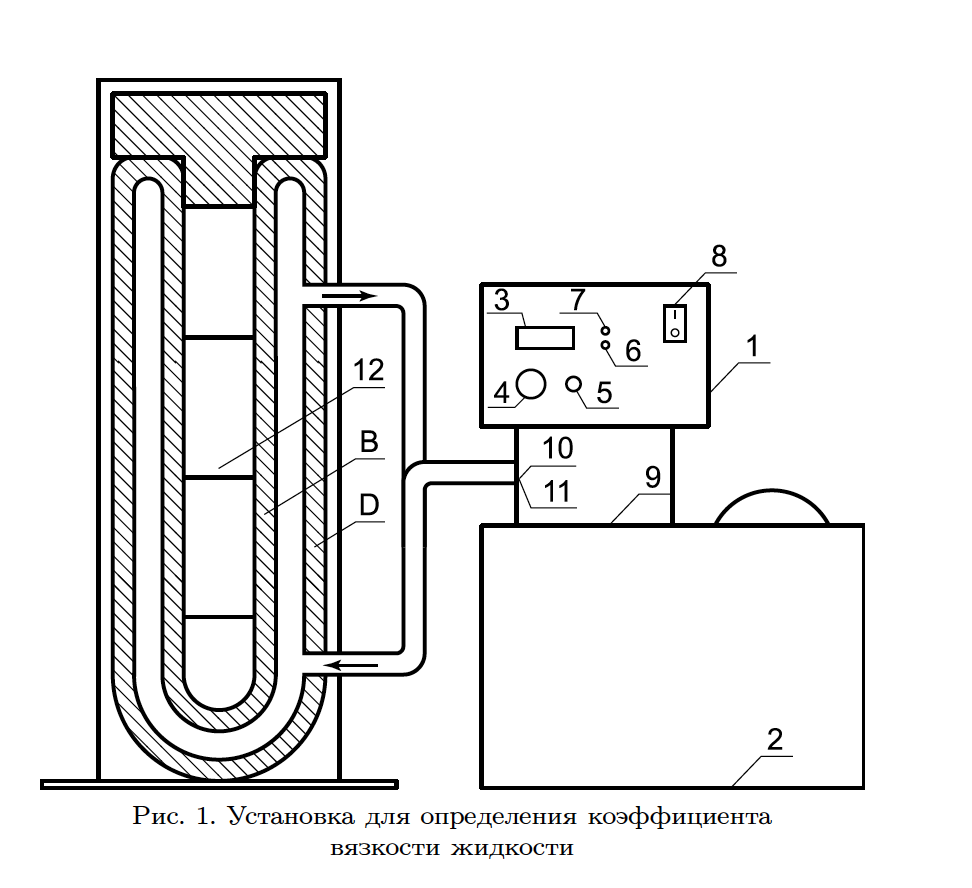
\includegraphics[width=0.5\textwidth]{226_ris1.png}
	%\caption{\label{fig:ris1} Установка для определения коэффициента вязкости жидкости}
	%\end{figure}
	
	\begin{figure}[h!]
		\begin{minipage}[h]{0.49\linewidth}
			\center{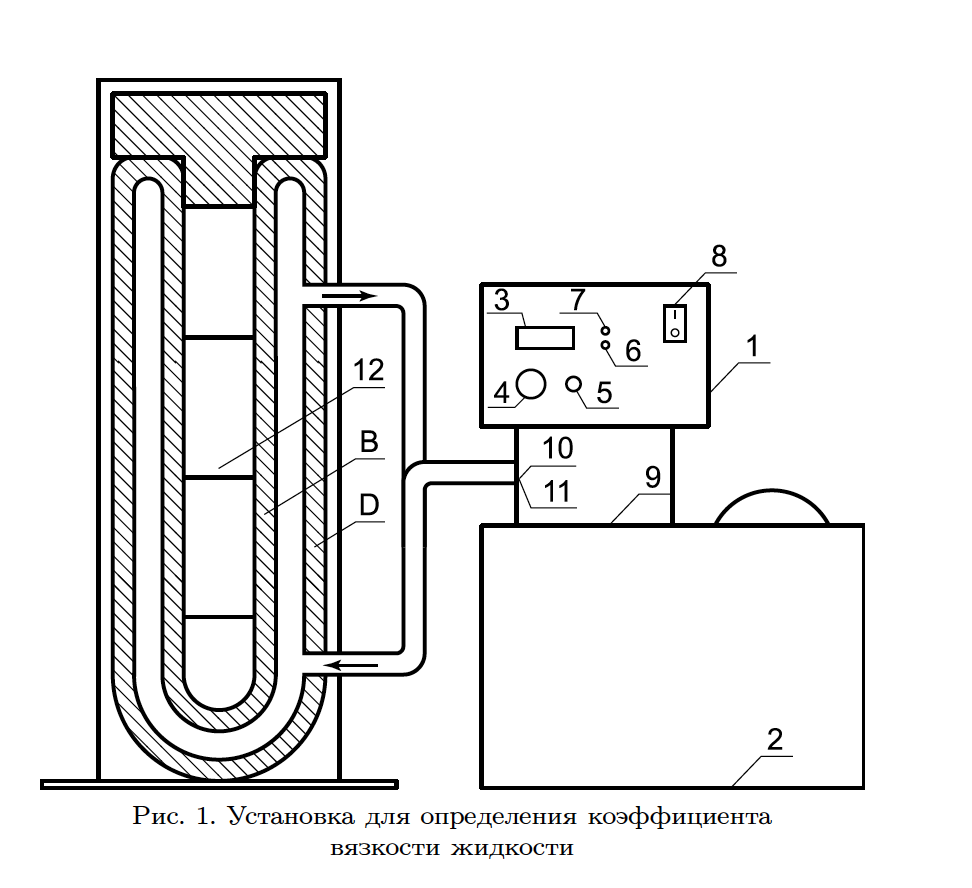
\includegraphics[width=0.6\linewidth]{226_ris1.png}}
		\end{minipage}
		\hfill
		\begin{minipage}[h!]{0.49\linewidth}
			\center{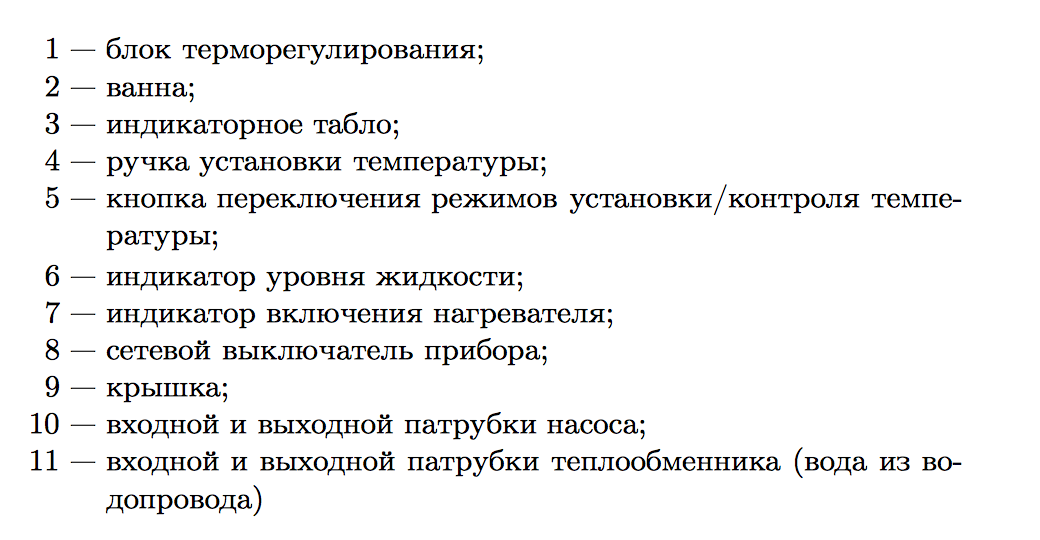
\includegraphics[width=0.9\linewidth]{226_ris2}}
		\end{minipage}
		\label{ris:image1}
	\end{figure}
	
	\section{Ход работы}
	1. Отобрали 18 шариков различного размера и с помощью микроскопа измерили их диаметры.
	\begin{table}[h]
		\parbox{.45\linewidth}{
			\centering
			\begin{tabular}{|c|c|} \hline
				№ & d, мм \\ \hline
				1 & 0,72 \\ \hline
				2 & 0,92 \\ \hline
				3 & 0,66 \\ \hline
				4 & 0,78 \\ \hline
				5 & 0,80 \\ \hline
				6 & 0,84 \\ \hline
				7 & 0,68 \\ \hline
				8 & 0,80 \\ \hline
				9 & 0,86 \\ \hline
			\end{tabular}
			\caption{Сталь, $\rho_\text{сталь}$ = 7,8 г/см^3 }
		}
		\hfill
		\parbox{.45\linewidth}{
			\centering
			\begin{tabular}{|c|c|} \hline
				№ & d, мм \\ \hline
				10 & 2,10 \\ \hline
				11 & 2,10 \\ \hline
				12 & 2,00 \\ \hline
				13 & 2,08 \\ \hline
				14 & 2,06 \\ \hline
				15 & 2,06 \\ \hline
				16 & 2,06 \\ \hline
				17 & 2,02 \\ \hline
				18 & 2,06 \\ \hline
			\end{tabular}
			\caption{Стекло, $\rho_\text{стекло}$ = 2,6  г/см^3 }
		}
	\end{table}
	
	
	2. Измерили установившиеся скорости падения шариков и вычислили вязкость $\eta$ по формуле (6).  Измерения выполнили для 4 значений температуры в интервале от комнатной до 55 \degres C. Для каждого значения температуры определили плотность жидкости $\rho_\text{ж}$ по графику $\rho_\text{ж}(T)$ , приложенному к работе:
	\begin{figure}[H!]
	\centering
	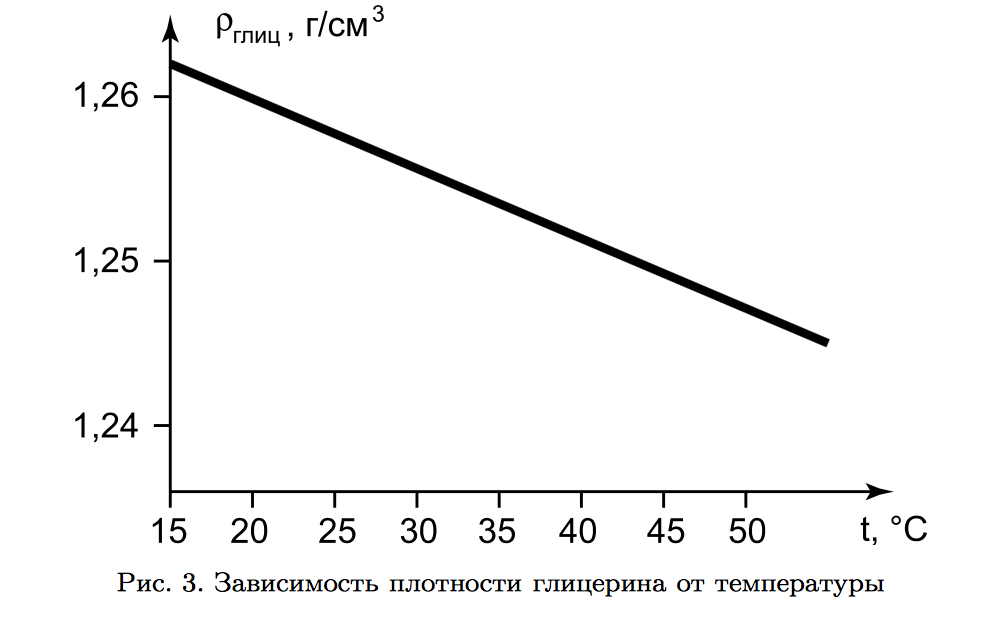
\includegraphics[width=0.5\textwidth]{226_ris3.png}
	\end{figure}

	%\hspace{10pt}
	\begin{table}[H!]
	\begin{adjustwidth}{-2cm}{}
		\scalebox{0.76}{\begin{tabular}{|c|c|c|c|c|c|c|c|c|c|c|c|c|c|c|c|c|c|c|} \hline
				T, K & \multicolumn{4}{|c|}{296,35} & \multicolumn{5}{|c|}{308,35} & \multicolumn{5}{|c|}{318,25}  & \multicolumn{4}{|c|}{328,15}  \\ \hline
				№ шарика & 1 & 5 & 11 & 12 & 2 & 4 & 6 & 10 & 15 & 3 & 8 & 13 & 16 & 18 & 7 & 9 & 14 & 17 \\ \hline
				d, мм & 0,72 & 0,80 & 2,10 & 2,06 & 0,92 & 0,78 & 0,84 & 2,10 & 2,06 & 0,66 & 0,80 & 2,00 & 2,06 & 2,06 & 0,68 & 0,86 & 2,08 & 2,02 \\ \hline
				$\rho$, г/см^{3} & 7,8 & 7,8  & 2,6 & 2,6 & 7,8 & 7,8 & 7,8 & 2,6 & 2,6 & 7,8 & 7,8 & 2,6 & 2,6 & 2,6 & 7,8 & 7,8 & 2,6 & 2,6 \\ \hline
				$\rho_\text{ж}$, г/см^{3} & \multicolumn{4}{|c|}{1,260} & \multicolumn{5}{|c|}{1,255} & \multicolumn{5}{|c|}{1,250}  & \multicolumn{4}{|c|}{1,246}  \\ \hline
				$r$, 10^{-3} м & 0,36 & 0,40 & 1,05 & 1,03 & 0,46 & 0,39 & 0,42 & 1,05 & 1,03 & 0,33 & 0,40 & 1,00 & 1,03 & 1,03 & 0,34 & 0,43 & 1,04 & 1,01 \\ \hline
				$r^{2}, 10^{-6}$ м^2 & 0,130 & 0,160 & 1,103 & 1,061 & 0,212 & 0,152 & 0,176 & 1,103 & 1,061 & 0,109 & 0,160 & 1,00 & 1,061 & 1,061 & 0,116 & 0,185 & 1,082 & 1,020 \\ \hline
				t, c & 18,44 & 14,59 & 13,02 & 13,09 & 9,8 & 11,01 & 9,19 & 7,69 & 7,44 & 8,41 & 5,27 & 4,84 & 4,5 & 4,71 & 4,03 & 3,22 & 2,72 & 2,61 \\ \hline
				$v_\text{уст}, 10^{-2} $ м/с & 0,542 & 0,685 & 0,768 & 0, 764 & 1,020 & 0,908 & 1,088 & 1,300 & 1,344 & 1,189 & 1,898 & 2,066 & 2,222 & 2,123 & 2,481 & 3,105 & 3,676 & 3,831  \\ \hline
				$\eta, 10^{-3}$ Па*c & 315 & 308 & 388 & 375 & 273 & 221 & 214 & 230 & 214 & 121 & 111 & 131 & 130 & 136 & 61 & 78 & 80 & 72  \\ \hline
				$<\eta>, 10^{-3}$ Па*c & \multicolumn{4}{|c|}{346,757} & \multicolumn{5}{|c|}{230,681} & \multicolumn{5}{|c|}{126,097}  & \multicolumn{4}{|c|}{73,365}  \\ \hline
				$Re$ & 0,008 & 0,011 & 0,026 & 0,026 & 0,022 & 0,020 & 0,027 & 0,074 & 0,081 & 0,040 & 0,085 & 0,196 & 0,220 & 0,201 & 0,170 & 0,211 & 0,593 & 0,663 \\ \hline
				$\tau$, c & 0,006 & 0,008 & 0,015 & 0,014 & 0,012 & 0,011 & 0,013 & 0,025 & 0,026 & 0,014 & 0,022 & 0,039 & 0,043 & 0,041 & 0,030 & 0,037 & 0,071 & 0,074 \\ \hline
				$S, 10^{-5}$ м & 1,289 & 2,060 & 4,208 & 4,163 & 4,562 & 3,614 & 5,188 & 12,02 & 12,84 & 6,190 & 15,76 & 30,02 & 34,96 & 31,92 & 26,94 & 42,20 & 95,42 & 103,6 \\ \hline
 		\end{tabular}}
		\caption{\label{tab:widgets} Измерения и результаты вычислений}
	\end{adjustwidth}
	\end{table}

	3.  Для каждого из опытов вычислили значение числа Рейнольдса $Re$, оценили время релаксации $\tau$ (по формуле (5)) и путь релаксации $S$, который может быть найден посредством интегрирования (4). Полагая для простоты $v(0) = 0$ (что обычно выполняется с достаточной точностью), получим
	\[ S = v_\text{уст} \tau (\frac{t}{\tau} - 1 + e^{-t/\tau}). \eqno(7)\]
	 При выводе формулы Стокса предполагалось, что обтекание шарика жидкостью имеет ламинарный характер. Как известно, характер обтекания определяется значением числа Рейнольдса $Re = v r \rho_\text{ж} / \eta$. Обтекание является ламинарным лишь при не очень больших значениях $Re (< 10)$. Следовательно, как видно по расчетам, в каждом эксперименте формула Стокса применима.
	
	4.  Построили график зависимости $ln\overline{\eta}$ от $1/T$ .
	\begin{table}[h]
	\centering
		\begin{tabular}{|c|c|c|c|c|} \hline
			$ln\overline{\eta} $ , Па*c & -1,059 & -1,467 & -2,071 & -2,612 \\ \hline
			$1/T, \frac{1}{K}*10^{-3}$ & 3,374 & 3,243 & 3,142 & 3,047 \\ \hline
		\end{tabular}
	\end{table}

	\begin{figure}[h!]
		\centering
		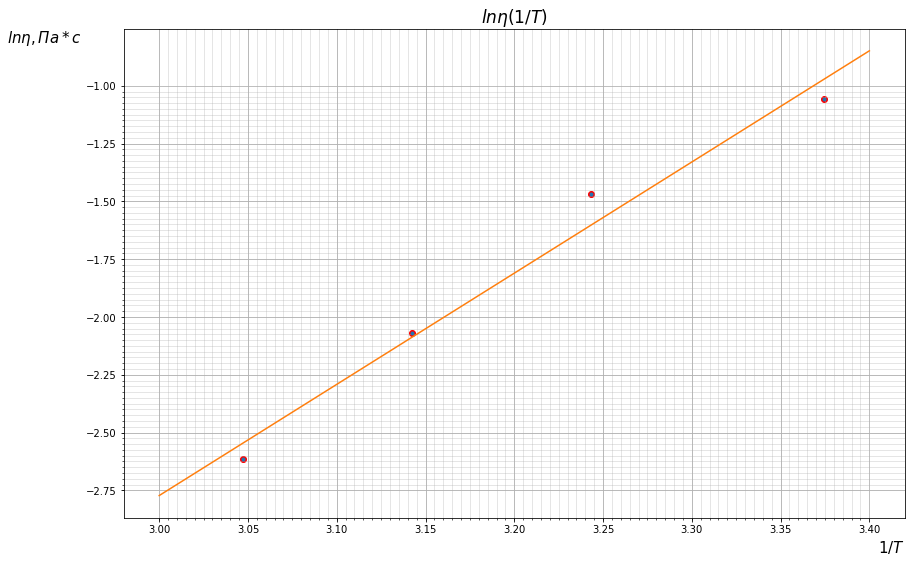
\includegraphics[width=1\textwidth]{226_ris4.png}
	\end{figure}
	Из (1) получаем выражения для энергии активации молекулы исследуемой жидкости:
	\[ W = k \frac{d(ln\eta)}{d(1/T)}. \]
	
	С помощью метода МНК вычислили: $\frac{d(ln\eta)}{d(1/T)} = (4,809 \pm 0,364) * 10^{3}$.

	Найдем энергию активацию глицерина и погрешности для нее:
	
	$W = k \frac{d(ln\eta)}{d(1/T)} = 1,38 * 10^{-23} * 10^{3} * (4,809 \pm 0,364) = (6,636 \pm 0,502) * 10^{-20}$ Дж
	
	
	
	\textbf{Вывод:} измерили скорости падения шариков при разной температуре глицерина, для каждого эксперимента вычислили значение вязкости глицерина; получили зависимость $ln\overline{\eta}$ от $1/T$, с помощью которой вычислили значение энергии активации глицерина; в пределах погрешнсости полученное значение не сходится со справочным ($8,341 * 10^{-20}$ Дж), однако же достаточно близко к нему (как минимум, имеет тот же порядок); возможно, полученное значение не сошлось со справочным, потому что при проведении эксперимента мы не достаточно выжидали, чтобы успело установиться термическое равновесие системы.
	

	
\end{document}